\documentclass[runningheads]{llncs}
\usepackage{xcolor}
\usepackage{url}
\usepackage{graphicx} 
\usepackage{amssymb}
\usepackage{amsmath}
\usepackage{tikz}
\usetikzlibrary{arrows.meta, positioning, fit}

\definecolor{uf_blue}{RGB}{17,27, 150}
\definecolor{uf_orange}{RGB}{150,100,17}

\begin{document}

\title{Learning to Dispatch: A Reinforcement Learning Framework for Train Networks}

\author{\textcolor{uf_blue}{Andres Espinosa}}
\institute{
    \textcolor{uf_orange}{Industrial and Systems Engineering \\
    University of Florida}\\
    \textcolor{uf_orange}{\email{andresespinosa@ufl.edu}}
}
\maketitle


\begin{abstract}

\end{abstract}



\section{Introduction}
\label{sse:introduction}

% What is the problem?
The Train Dispatching Problem (TDP) concerns the real-time management of train movements across a rail network, ensuring safe and efficient use of infrastructure. 
This involves deciding when and where trains should move, stop, or wait, based on factors such as schedules, track availability, and priority rules. 
Dispatching decisions must be made continuously and quickly, especially in high-traffic networks, making the problem both operationally critical and computationally challenging.

% Why does the problem exist?
Despite significant technological advances in other areas of transportation and logistics, train dispatching remains heavily reliant on human decision-makers or static rule-based systems. 
This is largely because the problem is highly combinatorial: at any given moment, there are exponentially many possible sequences of decisions that can lead to different network outcomes. 
Human dispatchers bring experience and intuition to these situations, but they are limited in how much information they can process and how consistently they can manage large-scale disruptions or optimize traffic flow over time.

% Why solve this problem?
Improving train dispatching systems has the potential to reduce passenger delays, minimize dispatching errors, and prevent network deadlocks—situations where no train can proceed without violating safety or scheduling constraints. 
Optimized dispatching can also improve energy efficiency and capacity utilization, making rail transport more competitive and sustainable. 
In dense urban transit systems or busy freight corridors, even marginal improvements in dispatching can lead to significant gains in overall network performance and reliability.

% Why solve with RL?
Reinforcement Learning (RL) offers a new approach to tackling the TDP by framing it as a sequential decision-making problem, where an agent learns to make dispatching decisions through interactions with a simulated environment. 
RL is particularly well-suited for problems with delayed consequences, dynamic environments, and large state spaces—all of which characterize train dispatching. 
With recent successes in games, robotics, and supply chain optimization, RL is emerging as a promising tool for learning policies that outperform hand-crafted heuristics in complex, real-world systems.

% Project scope.
This paper focuses on the formulation of the Train Dispatching Problem for RL-based approaches, rather than on developing a fully trained solution. 
We emphasize how the problem can be encoded as an RL task using graph structures to represent rail networks, define meaningful states, actions, and rewards, and manage constraints inherent to railway systems. 
Our goal is to provide a robust and extensible framework that future researchers and practitioners can build upon when applying RL methods to train dispatching and related infrastructure scheduling problems.

% Paper Outline
To provide a thorough understanding of our approach, the remainder of this paper is organized as follows. 
In Section~\ref{sse:background}, we present the foundational background necessary for our formulation, beginning with a formal description of the Train Dispatch Problem and its mixed-integer programming (MIP) formulation, as well as the DISPLIB benchmark format (\ref{sss:train}). 
We then outline key reinforcement learning concepts, including Markov Decision Processes (\ref{sss:reinforcement_learning}) and Deep Q-Networks, highlighting their relevance to sequential decision-making in dispatching tasks. This is followed by an introduction to Graph Neural Networks (\ref{sss:gnn}), which are critical for representing the structure of railway networks. 
Section~\ref{sse:related_work} provides a review of related literature, including recent RL applications to combinatorial scheduling, graph-based approaches, and prior work on train dispatching. 
Section~\ref{sse:formulation} details our proposed formulation, introducing Train Operation Graphs (\ref{sss:train_ops}), Resource Conflict Graphs (\ref{sss:resource_conflicts}), and the definitions of our state and action spaces (\ref{sss:state_space}, \ref{sss:action_space}). 
In Section~\ref{sse:results}, we demonstrate preliminary results from our Deep Graph Q-Network agent (\ref{sss:agent}), evaluating its performance on sample instances and visualizing its learned strategies (\ref{sss:solutions}). 
Finally, Section~\ref{sse:conclusion} outlines our conclusions and discusses future directions for scaling and refining the framework (\ref{sss:future_work}, \ref{sss:conclusion}).



\section{Problem Background}
\label{sse:background}
\subsection{Train Dispatch Problem}
\label{sss:train}
% This should cover the MIP formulation and the general outline of the problem
% This should also cover the DISPLIB data format and all that.
\subsection{Deep Reinforcement Learning}
\label{sss:reinforcement_learning}
% Cover Markov Decision Processes
% As well as DQN
\subsubsection{Markov Decision Processes}



\begin{figure}
    \centering
    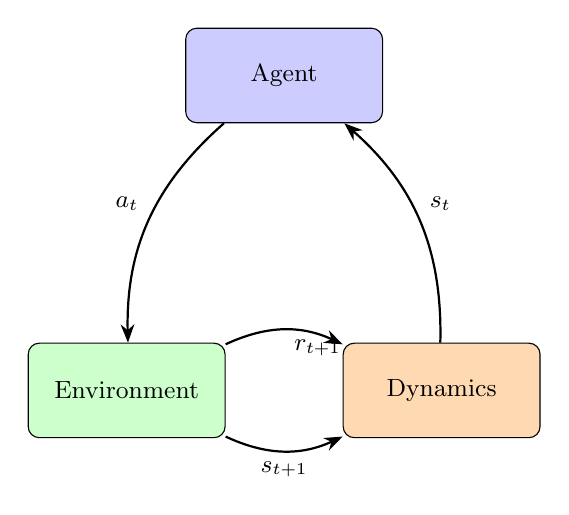
\begin{tikzpicture}[
      agent/.style={draw, rounded corners, fill=blue!20, minimum width=2.5cm, minimum height=1.2cm},
      env/.style={draw, rounded corners, fill=green!20, minimum width=2.5cm, minimum height=1.2cm},
      reward/.style={draw, rounded corners, fill=orange!30, minimum width=2.5cm, minimum height=1.2cm},
      arrow/.style={->, thick, >=Stealth},
      every node/.style={font=\small}
      ]
    
    % Nodes
    \node[agent] (agent) at (0, 2) {Agent};
    \node[env] (env) at (-2, -2) {Environment};
    \node[reward] (reward) at (2, -2) {Dynamics};
    
    % Arrows
    \draw[arrow] (agent) to[bend right=25] node[above left] {$a_t$} (env);
    \draw[arrow] (env) to[bend right=25] node[below] {$s_{t+1}$} (reward);
    \draw[arrow] (reward) to[bend right=25] node[above right] {$s_t$} (agent);
    \draw[arrow] (env) to[bend left=25] node[below right] {$r_{t+1}$} (reward);
    
    \end{tikzpicture}
    \caption{The reinforcement learning framework.}
    \label{fig:rl_framework}
\end{figure}

\subsubsection{Deep Q-Network}


\begin{figure}
    \centering
    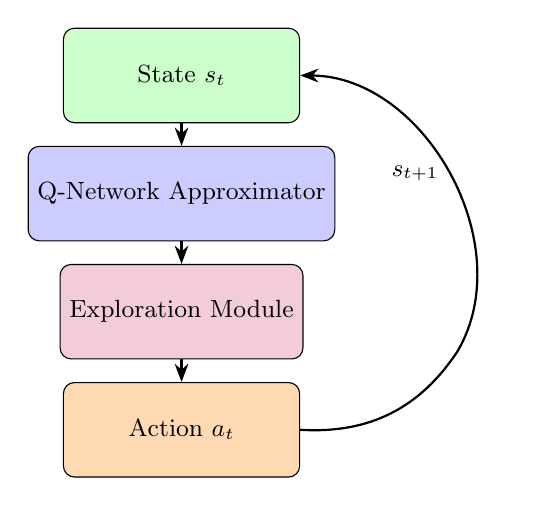
\begin{tikzpicture}[
      qnet/.style={draw, rounded corners, fill=blue!20, minimum width=3cm, minimum height=1.2cm},
      module/.style={draw, rounded corners, fill=purple!20, minimum width=3cm, minimum height=1.2cm},
      action/.style={draw, rounded corners, fill=orange!30, minimum width=3cm, minimum height=1.2cm},
      state/.style={draw, rounded corners, fill=green!20, minimum width=3cm, minimum height=1.2cm},
      arrow/.style={->, thick, >=Stealth},
      every node/.style={font=\small}
    ]
    
    % Nodes
    \node[state] (state) at (0, 2) {State $s_t$};
    \node[qnet] (qnet) at (0, 0.5) {Q-Network Approximator};
    \node[module] (explore) at (0, -1) {Exploration Module};
    \node[action] (action) at (0, -2.5) {Action $a_t$};
    
    % Arrows
    \draw[arrow] (state) -- (qnet);
    \draw[arrow] (qnet) -- (explore);
    \draw[arrow] (explore) -- (action);
    \draw[arrow] (action.east) to[bend right=30] node[right] {} ++(2,1) 
        to[bend right=60] node[left] {$s_{t+1}$} (state.east);

    \end{tikzpicture}
    \caption{The Deep Q-Network action selection and feedback loop.}
    \label{fig:dqn_loop}
\end{figure}



\subsection{Graph Neural Networks}
\label{sss:gnn}
% Cover graph neural networks

\section{Related Work}
\label{sse:related_work}
% This can be a full literature review following the structure of:
% 1) Train Dispatch Problem Formulation
% 2) Deep Reinforcement Learning with similar problems
% 3) Graph Neural Networks
I am \cite{gnndrl:Devailly_2022}
\section{Formulation}
\label{sse:formulation}

\subsection{Train Operation Graphs}
\label{sss:train_ops}


\subsection{Resource Conflict Graphs}
\label{sss:resource_conflicts}


\subsection{State Space}
\label{sss:state_space}

\subsection{Action Space}
\label{sss:action_space}

\section{Preliminary Agent Results}
\label{sse:results}

\subsection{Deep Graph Q-Network Agent}
\label{sss:agent}


\subsection{Solutions}
\label{sss:solutions}


\section{Conclusion and Future Work}
\label{sse:conclusion}

\subsection{Future Work}
\label{sss:future_work}

\subsection{Conclusion}
\label{sss:conclusion}


\section{Appendix}

\begin{figure}
    \centering
    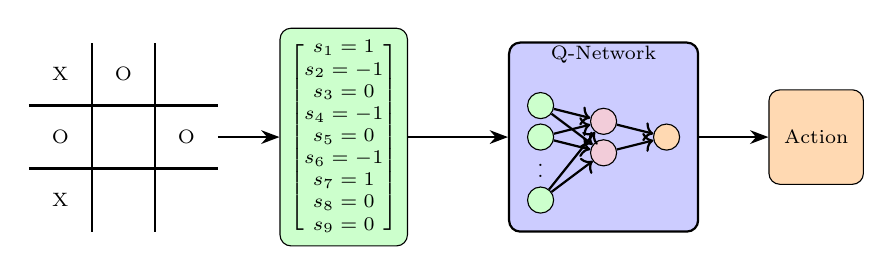
\begin{tikzpicture}[
        qnet/.style={draw, rounded corners, fill=blue!20, minimum width=1.2cm, minimum height=1.2cm},
        module/.style={draw, rounded corners, fill=purple!20, minimum width=1.2cm, minimum height=1.2cm},
        action/.style={draw, rounded corners, fill=orange!30, minimum width=1.2cm, minimum height=1.2cm},
        state/.style={draw, rounded corners, fill=green!20, minimum width=1.2cm, minimum height=1.2cm},
        arrow/.style={->, thick, >=Stealth},
        every node/.style={font=\scriptsize}
      ]
        % Vertical lines
        \draw[thick] (0.8,0) -- (0.8,2.4);
        \draw[thick] (1.6,0) -- (1.6,2.4);
        % Horizontal lines
        \draw[thick] (0,0.8) -- (2.4,0.8);
        \draw[thick] (0,1.6) -- (2.4,1.6);
        
        % Xs and Os
        \node at (0.4, 2) {X};
        \node at (1.2, 2) {O};
        \node at (2, 2) {};
        \node at (0.4, 1.2) {O};
        \node at (1.2, 1.2) {};
        \node at (2, 1.2) {O};
        \node at (0.4, 0.4) {X};
        \node at (1.2, 0.4) {};
        \node at (2, 0.4) {};

        \node[state] (state) at (4,1.2) {
            $\begin{bmatrix}
            s_1 = 1 \\ s_2 = -1 \\ s_3 = 0 \\ s_4 = -1 \\ s_5 = 0 \\ s_6 = -1 \\ s_7 = 1 \\ s_8 = 0 \\ s_9 = 0
            \end{bmatrix}$
        };
        \draw[arrow] (2.4,1.2) -- (state);

        \begin{scope}[shift={(6.5, 2)}]
            % Box and title
            \node[draw, rounded corners, thick, fill=blue!20, fit={(0, -1.6) (1.6, 0)}, inner sep=0.4cm, label={[yshift=-0.4cm]above:Q-Network}] (box) {};
            
            % Input layer
            \foreach \i in {1, 2} {
                \node[circle, draw, fill=green!20, minimum size=0.3cm] (input\i) at (0, -\i*0.4) {};
            }
            \node at (0, -1.2) {$\vdots$};
            \node[circle, draw, fill=green!20, minimum size=0.3cm] (input3) at (0, -1.6) {};
            
            % Hidden layer
            \foreach \i in {1, 2} {
                \node[circle, draw, fill=purple!20, minimum size=0.3cm] (hidden\i) at (0.8, -\i*0.4-0.2) {};
            }
            
            % Output layer
            \node[circle, draw, fill=orange!30, minimum size=0.3cm] (output) at (1.6, -0.8) {};
            
            % Connections
            \foreach \i in {1, 2, 3} {
                \foreach \j in {1, 2} {
                    \draw[->, thick] (input\i) -- (hidden\j);
                }
            }
            \foreach \i in {1, 2} {
                \draw[->, thick] (hidden\i) -- (output);
            }
        \end{scope}
        \draw[arrow] (state) -- (box);

        \node[action] (action) at (10, 1.2) {Action};

        \draw[arrow] (box) -- (action);
        
    \end{tikzpicture}
    \caption{Illustration of a Q-Network processing a Tic-Tac-Toe board state.}
    \label{fig:qnetwork_tictactoe}
\end{figure}




\bibliographystyle{IEEEtran}
\bibliography{references}  % Assuming your .bib file is named references.bib


\end{document}



